\documentclass[11pt]{article}
\usepackage[utf8]{inputenc} 

%%% PAGE DIMENSIONS
\usepackage{geometry}
\geometry{a4paper}

\usepackage{graphicx}

%%% PACKAGES
\usepackage{booktabs}
\usepackage{paralist}
\usepackage{verbatim}
\usepackage{subfig}
\usepackage{chngcntr}
\usepackage{tikz}
\usepackage[colorlinks = true,
            linkcolor = black,
            urlcolor  = blue,
            citecolor = blue,
            anchorcolor = blue]{hyperref}
\usepackage[spanish]{cleveref}

%%% HEADERS & FOOTERS
\usepackage{fancyhdr}
\pagestyle{fancy}
\renewcommand{\headrulewidth}{0pt}
\lhead{}\chead{}\rhead{}
\lfoot{}\cfoot{\thepage}\rfoot{}

%%% SECTION TITLE APPEARANCE
\usepackage{sectsty}
\allsectionsfont{\sffamily\mdseries\upshape}

%%% ToC (table of contents) APPEARANCE
\usepackage[nottoc,notlof,notlot]{tocbibind} % Put the bibliography in the ToC
\usepackage[titles,subfigure]{tocloft} % Alter the style of the Table of Contents
\renewcommand{\cftsecfont}{\rmfamily\mdseries\upshape}
\renewcommand{\cftsecpagefont}{\rmfamily\mdseries\upshape} % No bold!


\graphicspath{ {images/} }

\counterwithin*{figure}{section}
\counterwithin*{figure}{subsection}
\counterwithin*{figure}{subsubsection}

\counterwithin*{table}{section}
\counterwithin*{table}{subsection}
\counterwithin*{table}{subsubsection}

\addtolength{\cftfignumwidth}{2em}

\renewcommand{\thefigure}{
  \ifnum\value{subsection}=0
    \thesection.\arabic{figure}
  \else
    \ifnum\value{subsubsection}=0
      \thesubsection.\arabic{figure}
    \else
      \thesubsubsection.\arabic{figure}
    \fi
  \fi
}

\renewcommand{\thetable}{
  \ifnum\value{subsection}=0
    \thesection.\arabic{table}
  \else
    \ifnum\value{subsubsection}=0
      \thesubsection.\arabic{table}
    \else
      \thesubsubsection.\arabic{table}
    \fi
  \fi
}

%%% END Article customizations

%%% The "real" document content comes below...

\title{\Large Seguridad en Redes\\Practica 2.1}
\author{David Antuña Rodríguez\\Javier Carrión García}
\date{}

\begin{document}
  \raggedright

  \maketitle
  \newpage

  \section{OpenSSL}
    \subsection{Cifrado de bloque}
      \par
      Los textos generados no son iguales porque la clave de cifrado del algoritmo es distinta a pesar de que las contraseñas coincidan.
      \begin{figure}[!h]
        \centering
        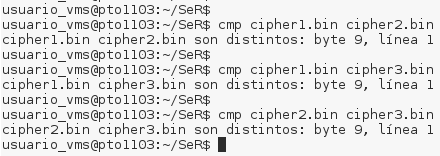
\includegraphics[width = .6\textwidth]{cmp_ciphers}
        \caption{Comparación de los ficheros generados.}
      \end{figure}

      \bigskip
      \par
      Por defecto OpenSSL utiliza salt al derivar la clave de cifrado para evitar los ataques por diccionario. Al utilizar la
      opción no salt se elimina el componente aleatorio de la clave, la salt, por lo que la misma clave da lugar al mismo texto cifrado.
      \begin{figure}[!h]
        \centering
        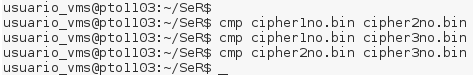
\includegraphics[width = .7\textwidth]{cmp_ciphers_nosalt}
        \caption{Comparación de los cifrados sin salt.}
      \end{figure}

      \par
      Al cifrar o descifrar con OpenSSL se pueden utilizar las siguientes opciones.
      \begin{itemize}
        \item \textbf{-p}: muestra la key e iv usados para cifrar/descifrar.
              \begin{figure}[!h]
                \centering
                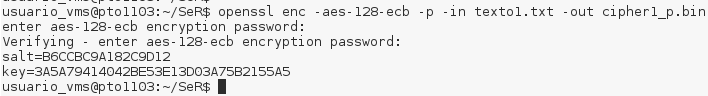
\includegraphics[width = .9\textwidth]{cipher_p}
                \caption{Cifrado utilizando la opcion -p.}
              \end{figure}
              \begin{figure}[!h]
                \centering
                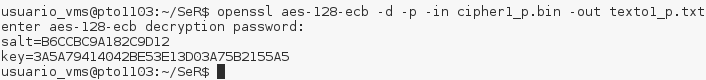
\includegraphics[width = .9\textwidth]{dcipher_p}
                \caption{Descifrado utilizando la opcion -p.}
              \end{figure}
        \item \textbf{-P}: muestra la key e iv generados por no se llega a cifrar/descifrar.
        \item \textbf{-pass}: si no se quiere que openSSL solicite la clave por consola se puede utilizar esta opcion para indicar el origen de la misma.
              \begin{figure}[!h]
                \centering
                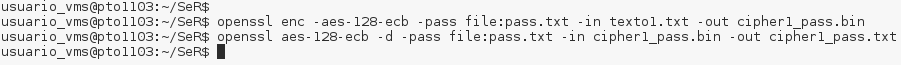
\includegraphics[width = .9\textwidth]{cipher_pass}
                \caption{Cifrado/descifrado utilizando la opcion -pass.}
              \end{figure}
        \item \textbf{-S}: permite especificar un salt, debe ser una cadena de digitos hexadecimales.
              \begin{figure}[!h]
                \centering
                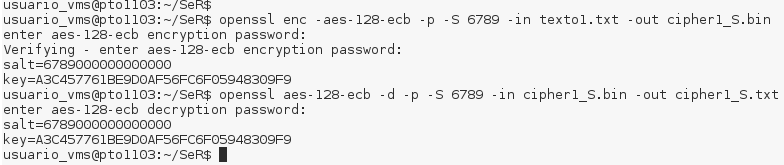
\includegraphics[width = .9\textwidth]{cipher_S}
                \caption{Cifrado/descifrado utilizando la opcion -S.}
              \end{figure}
        \item \textbf{-K}: permite especificar la key a utilizar, debe ser una cadeba de digitos hexadecimales. Obliga a utlizar tambien la opción-iv, porque el iv se genera al generar la key.
        \item \textbf{-iv}: permite especificar el iv a utilizar, debe ser una cadeba de digitos hexadecimales. Si se especifica se ignora el iv que genere el proceso de creacion de la key, salvo que se hayan utilizado opciones especiales de generacion de la key.
              \begin{figure}[!h]
                \centering
                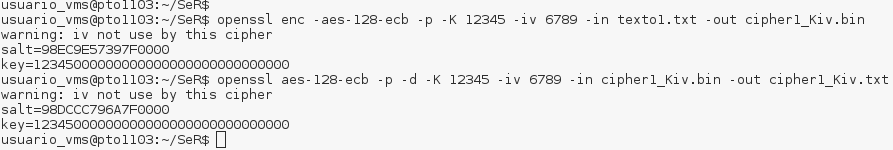
\includegraphics[width = .9\textwidth]{cipher_Kiv}
                \caption{Cifrado/descifrado utilizando las opciones -K y -iv.}
              \end{figure}
      \end{itemize}

      \par
      El receptor recibe la salt en el propio mensaje cifrado, \cref{fig:salt}, y obtiene el iv al generar la clave con dicha salt y la contraseña privada que ha de conocer.
      \begin{figure}[!h]
        \centering
        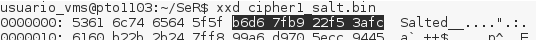
\includegraphics[width = .9\textwidth]{salt}
        \caption{Salt en el texto cifrado.}
        \label{fig:salt}
      \end{figure}

    \subsection{Modos de bloque}
      \par
      La diferencia es que en ecb podemos discernir los contornos de la figura y en cbc no se ve nada. Esto ocurre porque ecb no oculta los patrones del fichero origen en el fichero cifrado y cbc si.
      \begin{figure}[!h]
        \begin{minipage}[c]{.5\textwidth}
          \centering
          
\includegraphics[width = .8\textwidth]{tux-cbc}
          \caption{Cifrado con cbc.}
        \end{minipage}%
        \begin{minipage}[c]{.5\textwidth}
          \centering
          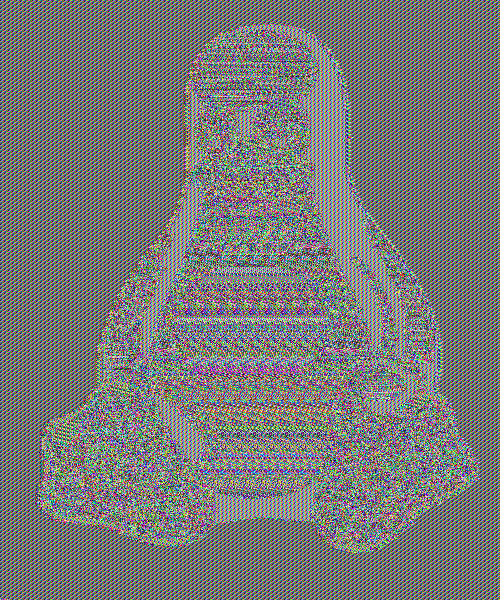
\includegraphics[width = .8\textwidth]{tux-ecb}
          \caption{Cifrado con ecb.}
        \end{minipage}
      \end{figure}

    \subsection{Cifrado de flujo}
      \par
      El texto en claro es \textbf{Attack at dawn}, la clave es \textbf{Secre} para el algoritmo compilado o \textbf{5365637265} para OpenSSL. Ambas claves son la misma pero a OpenSSL hay que proporcionarsela
      en hexadecimal y al compilado se le da la cadena.
      \par
      Usar :\\
      ./rc4 "Attack at dawn" "Secre"\\
      echo ‐ne "Attack at dawn" $\mid$ openssl enc ‐rc4‐40 ‐K 5365637265 $\mid$ xxd –u ‐p

      \begin{figure}[!h]
        \centering
        %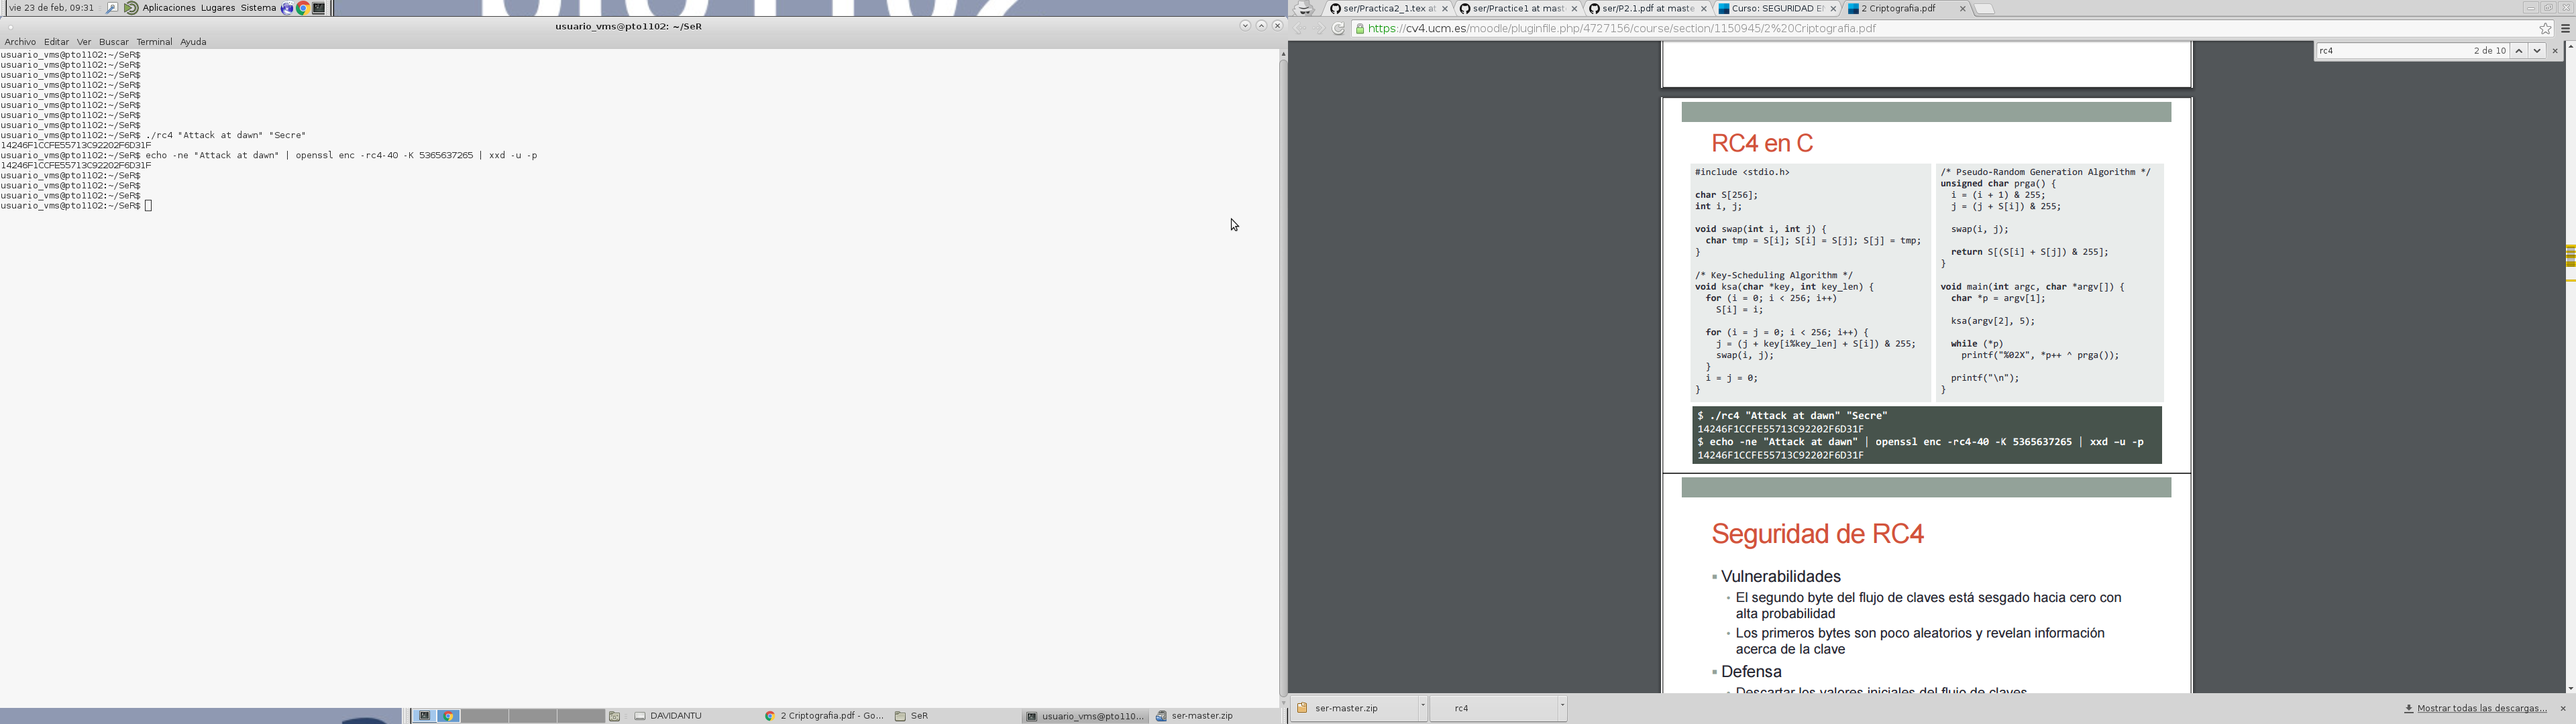
\includegraphics[width = .9\textwidth]{cipher_rc4}
        \caption{Cifrado con rc4-40.}
      \end{figure}

    \subsection{Funciones hash y HMAC}
      \par
      Se ha realizado el resumen de \textit{/etc/services} que tiene un tamaño de TODO.

      \par
      Usar:\\
      ls -l /etc/services\\
      openssl dgst -md5 /etc/services\\
      openssl dgst -sha1 /etc/services\\
      openssl dgst -sha256 /etc/services\\

      \begin{figure}[!h]
        \centering
        %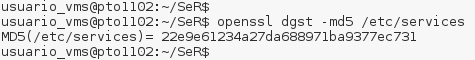
\includegraphics[width = .9\textwidth]{hash_md5}
        \caption{Hash utilizando md5.}
      \end{figure}

      \begin{figure}[!h]
        \centering
        %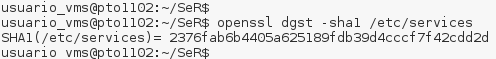
\includegraphics[width = .9\textwidth]{hash_sha1}
        \caption{Hash utilizando sha1.}
      \end{figure}

      \begin{figure}[!h]
        \centering
        %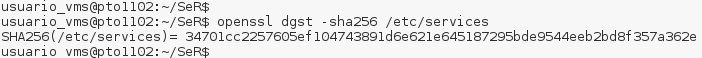
\includegraphics[width = .9\textwidth]{hash_sha256}
        \caption{Hash utilizando sha256.}
      \end{figure}

      \bigskip
      \par
      El valor del HMAC depende de la clave utilizada y la función de hash escogidas.
      Se han obtenido los siguientes HMAC del fichero \textit{/etc/services}.

      \par
      Usar:\\
      ls -l /etc/services\\
      openssl dgst -md5 -hmac seguridad /etc/services\\
      openssl dgst -sha1 -hmac seguridad /etc/services\\
      openssl dgst -sha256 -hmac seguridad /etc/services\\

      \begin{figure}[!h]
        \centering
        %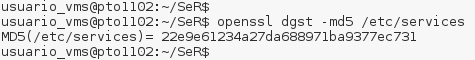
\includegraphics[width = .9\textwidth]{hash_md5}
        \caption{HMAC utilizando md5.}
      \end{figure}

      \begin{figure}[!h]
        \centering
        %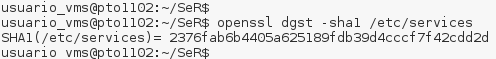
\includegraphics[width = .9\textwidth]{hash_sha1}
        \caption{HMAC utilizando sha1.}
      \end{figure}

      \begin{figure}[!h]
        \centering
        %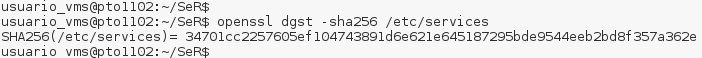
\includegraphics[width = .9\textwidth]{hash_sha256}
        \caption{HMAC utilizando sha256.}
      \end{figure}

  \section{GnuPG}
    \subsection{Cifrado y descifrado}
      \par
      Se ha cifrado el fichero \textit{/etc/services} utilizado la clave seguridad con \textbf{batch mode}, modo por bloques.

      \par
      Usar:\\
      cp /etc/services \$HOME/services\\
      gpg2 $--$version \hspace{10mm}y escoger uno de los algoritmos\\
      gpg2 $--$symmetric $--$cipher-algo $<$algoritmo escogido$>$ -a \$HOME/services

    \subsection{Funciones hash}
      \par
      Se ha calculado el hash de \textit{/etc/services} con varios algorimos.

      \par
      Usar:\\
      cp /etc/services \$HOME/services\\
      gpg2 $--$version \hspace{10mm}y escoger uno de los algoritmos\\
      gpg2 $--$symmetric $--$cipher-algo $<$algoritmo escogido$>$ -a \$HOME/services

      \begin{figure}[!h]
        \centering
        %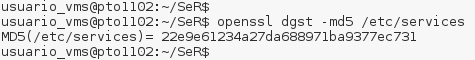
\includegraphics[width = .9\textwidth]{hash_md5}
        \caption{Hash utilizando .}
      \end{figure}

      \begin{figure}[!h]
        \centering
        %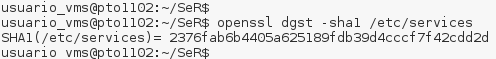
\includegraphics[width = .9\textwidth]{hash_sha1}
        \caption{Hash utilizando .}
      \end{figure}

      \begin{figure}[!h]
        \centering
        %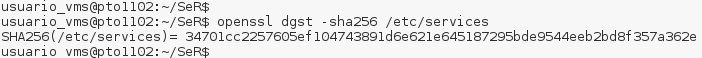
\includegraphics[width = .9\textwidth]{hash_sha256}
        \caption{Hash utilizando .}
      \end{figure}




\end{document}
